
\chapter{Introducción a la optimización de funcionales}

    El problema que tratamos de resolver es el siguiente; determinar $v(t)$, tal que la siguiente ecuación:

    \begin{equation} \label{eq:opfun1}
        J(v(t), v'(t)) = \int_{t_1}^{t_2} f_1(v(t), v'(t), t) dt
    \end{equation}

    sea un extremo.

    Primero definamos una función de vecindad $v(t) \to v(\alpha, t)$ tal que si $\alpha = 0 \implies v^* = v(0, t) = v(t)$, es decir, $v^*$ es la función que extremiza a $J(v(t), v'(t))$.

    Proponemos una solución en forma lineal:

    \begin{equation}
        v(\alpha, t) = v(0, t) + \alpha \eta(t)
    \end{equation}

    pero $v(t)$ y $u(t)$ deben ser idénticos en los puntos extremos.

    \begin{figure}
        \centering
        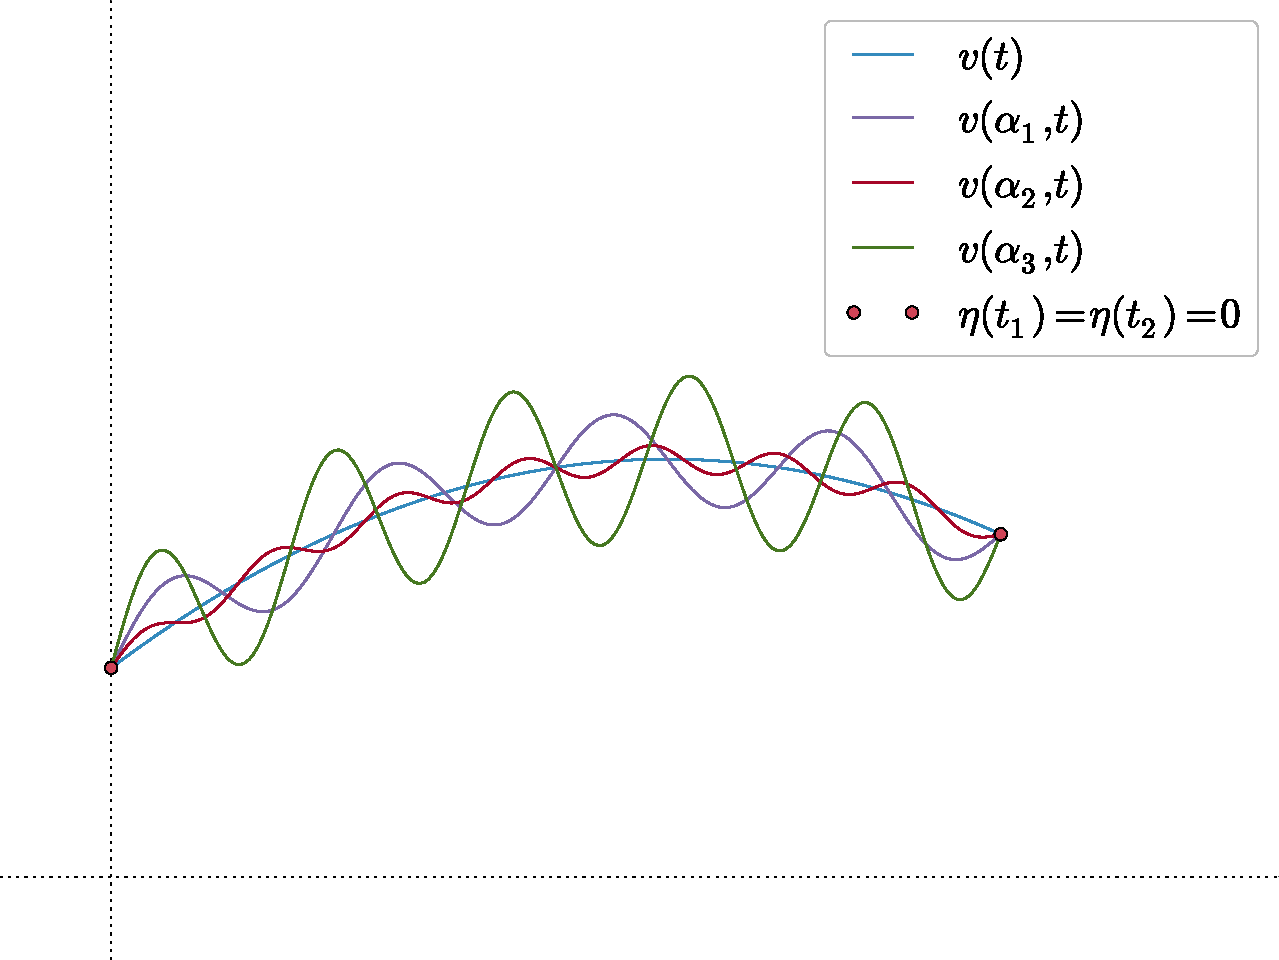
\includegraphics[width=0.7\textwidth]{./imagenes/trayectorias.pdf}
        \caption{\label{fig:trayectorias}Trayectorias $v(\alpha, t)$ solución para $J(v(t), v'(t))$.}
    \end{figure}

    es decir $\eta(t_1) = \eta(t_2) = 0$, pero además $\eta(t) \in e^1$.\footnote{Si $f \in e^1$, $f$ es una función diferenciable al menos una vez.}

    Con esta parametrización en $\alpha$:

    \begin{equation*}
        v(t) \to v(\alpha, t) = v(0, t) + \alpha \eta(t)
    \end{equation*}

    tenemos que la ecuación~\ref{eq:opfun1} nos queda:

    \begin{equation*}
        J(\alpha) = \int_{t_1}^{t_2} f_1(v(\alpha, t), v'(\alpha, t), t) dt
    \end{equation*}

    donde tenemos que $\alpha = 0$ implica que $J$ es un extremo y $\alpha \ne 0$ implica que $J$ no es un extremo.

    Debido a esto, podemos concluir que $J$ tambien esta parametrizada de esta manera:

    \begin{equation*}
        J \to J(\alpha)
    \end{equation*}

    La condición necesaria para que $J$ tenga un valor estacionario (extremo), es que $J$ sea independiente de $\alpha$ en primer orden (que este relacionado linealmente), a lo largo de la trayectoria que otorga el extremo ($\alpha = 0$), es decir:

    \begin{equation}
        \left. \frac{\partial J}{\partial \alpha} \right|_{\alpha=0} = 0 \quad \forall \eta \in e^1
    \end{equation}

    \begin{nota}
        Observe que solo es una condición necesaria, es decir:

        \begin{equation*}
            J \text{ es extremo } \implies \left. \frac{\partial J}{\partial \alpha} \right|_{\alpha=0} = 0
        \end{equation*}
    \end{nota}

    \newpage
    \section{Ecuación de Euler}

        La condición necesaria es:

        \begin{equation*}
            \left. \frac{\partial J}{\partial \alpha} \right|_{\alpha=0} = 0
        \end{equation*}

        entonces hay que seguir los siguientes pasos:

        \begin{enumerate}
            \item Calcular $\frac{\partial J}{\partial \alpha}$.
            \item Hacer $\alpha = 0$.
        \end{enumerate}

        Empecemos calculando la derivada parcial de $J$:

        \begin{multline*}
            \frac{\partial J}{\partial \alpha} = \frac{\partial}{\partial \alpha} \int_{t_1}^{t_2} f_1(v(\alpha, t), v'(\alpha, t), t)dt = \\
            \int_{t_1}^{t_2}\left( \frac{\partial f_1(\dots)}{\partial v(\alpha, t)} \frac{\partial v(\alpha, t)}{d \alpha} + \frac{\partial f_1(\dots)}{\partial v'(\alpha, t)} \frac{\partial v'(\alpha, t)}{d \alpha} \right) dt
        \end{multline*}

        en este punto aparecen términos reducibles:

        \begin{equation*}
            \frac{\partial v(\alpha, t)}{\partial \alpha} = \frac{\partial v(t)}{\partial \alpha} + \frac{\partial \left(\alpha \eta(t) \right)}{\partial \alpha} = \eta(t)
        \end{equation*}

        \begin{equation*}
            \frac{d v'(\alpha, t)}{d\alpha} = \frac{\partial}{\partial \alpha} \left( \frac{d v(\alpha, t)}{dt} \right) = \frac{\partial}{\partial \alpha} \left( v'(t) + \alpha \frac{d \eta(t)}{dt} \right) = \frac{d \eta(t)}{dt}
        \end{equation*}

        lo que nos deja:

        \begin{equation*}
            \frac{\partial J}{\partial \alpha} = \int_{t_1}^{t_2}\left( \frac{\partial f_1(\dots)}{\partial v(\alpha, t)} \eta(t) + \frac{\partial f_1(\dots)}{\partial v'(\alpha, t)} \frac{d \eta(t)}{dt} \right) dt
        \end{equation*}

        la segunda parte de esta integral es integrable por partes, si hacemos $u = \frac{\partial f_1(\dots)}{\partial v'(\alpha, t)}$, $dv = \frac{d\eta(t)}{dt}dt$, $du = \frac{d}{dt}\left( \frac{\partial f_1(\dots)}{dv'(\alpha, t)} \right)$ y $v = \eta(t)$:

        \begin{equation*}\frac{\partial J}{\partial \alpha} = \int_{t_1}^{t_2}\left( \frac{\partial f_1(\dots)}{\partial v(\alpha, t)} \eta(t) - \frac{d}{dt} \left( \frac{\partial f_1(\dots)}{\partial v'(\alpha, t)} \right) \eta(t) \right) dt + \left. \frac{\partial f_1(\dots)}{\partial v'(\alpha, t)} \eta(t) \right|_{t_1}^{t_2}
        \end{equation*}

        pero recordemos que $\eta(t_1) = \eta(t_2) = 0$, por lo que el ultimo termino se elimina y nos queda:

        \begin{multline} \label{eq:opfun2}
            \frac{\partial J}{\partial \alpha} = \int_{t_1}^{t_2}\left( \frac{\partial f_1(\dots)}{\partial v(\alpha, t)} \eta(t) - \frac{d}{dt} \left( \frac{\partial f_1(\dots)}{\partial v'(\alpha, t)} \right) \eta(t) \right) dt = \\
            \int_{t_1}^{t_2}\left( \frac{\partial f_1(v(\alpha, t), v'(\alpha, t), t)}{\partial v(\alpha, t)} - \frac{d}{dt} \left( \frac{\partial f_1(v(\alpha, t), v'(\alpha, t), t)}{\partial v'(\alpha, t)} \right) \right) \eta(t) dt
        \end{multline}

        Si ahora, en la ecuación~\ref{eq:opfun2} sustituimos $\alpha = 0$, obtendremos:

        \begin{equation*}
            \left. \frac{\partial J}{\partial \alpha} \right|_{\alpha=0} = \int_{t_1}^{t_2}\left( \frac{\partial f_1(v(t), v'(t), t)}{\partial v(t)} - \frac{d}{dt} \left( \frac{\partial f_1(v(t), v'(t), t)}{\partial v'(t)} \right) \right) \eta(t) dt
        \end{equation*}

        Por lo que la condición necesaria es:

        \begin{equation*}
            \int_{t_1}^{t_2}\left( \frac{\partial f_1(v(t), v'(t), t)}{\partial v(t)} - \frac{d}{dt} \left( \frac{\partial f_1(v(t), v'(t), t)}{\partial v'(t)} \right) \right) \eta(t) dt = 0 \quad \forall \eta(t) \in e^1
        \end{equation*}

        lo cual implica que:

        \begin{equation}
            \frac{\partial f_1(v(t), v'(t), t)}{\partial v(t)} - \frac{d}{dt} \left( \frac{\partial f_1(v(t), v'(t), t)}{\partial v'(t)} \right)  = 0
        \end{equation}

        esta es la que conocemos como ecuación de Euler.

    \newpage
    \section{Multiplicadores de Lagrange}

        Deseamos resolver el siguiente problema:

        Minimizar la función
        $f(v):\mathbbm{R}^n \to \mathbbm{R}$
        sujeta a la restricción $\mathscr{G}(v) = 0$
        , donde $\mathscr{G}(v)=\begin{pmatrix}\mathscr{G}_1(v) & \mathscr{G}_2(v) & \dots & \mathscr{G}_m(v) \end{pmatrix} \in \mathbbm{R}^m$
         y $\mathscr{G}_i(v): \mathbbm{R}^n \to \mathbbm{R}$
         con $i \in \left\{ 1, 2, \dots, m \right\}$.

        Para resolver este problema haremos uso de los multiplicadores de Lagrange, los cuales estan basados en el concepto de la derivada direccional\footnote{Esta derivada es formalmente conocida como la derivada de Fréchet, la cual se relaciona linealmente con la diferencial de Fréchet.}

        \subsection{Derivada direccional y vector gradiente}

            \begin{definicion}
                La derivada direccional de $f_1$ en $v_0 \in \mathbbm{R}^n$ en la dirección del vector unitario $\eta \in \mathbbm{R}^n$ es:

                \begin{equation}
                    D_{\eta} f_1(v_0) = \lim_{\alpha \to 0}^{n}  \frac{f_1(v_0 + \alpha) - f_1(v_0)}{\alpha}
                \end{equation}

                donde $\alpha$ es un escalar, es decir, $\alpha \in \mathbbm{R}$, en el caso de que este limite exista.

                \missingfigure{Superficie con vector posición evaluado y vector dirección de la derivada unitario.}

                \missingfigure{Curva cortada por una recta por la que pasa un vector restando los dos puntos evaluados de la curva.}

                Esta derivada nos da la razon de cambio de $f_1$ en el punto $v_0$ y en la dirección $\eta$, siempre y cuando $\alpha \to 0$.
            \end{definicion}

            \begin{teorema}
                Si $f_1$ es una función diferenciable de $v \in \mathbbm{R}^n$, entonces $f_1$ tiene una derivada direccional en la dirección de cualquier vector unitario $\eta \in \mathbbm{R}^n$ y por lo tanto:

                \begin{equation}
                    D_{\eta} f_1(v) = \sum_{i=1}^n \frac{\partial f_1(v_i)}{dv_i} \eta_i
                \end{equation}

                donde $v = \begin{pmatrix} v_1 \\ v_2 \\ \vdots \\ v_n \end{pmatrix} \in \mathbbm{R}^n$, $\eta = \begin{pmatrix} \eta_1 \\ \eta_2 \\ \vdots \\ \eta_n \end{pmatrix} \in \mathbbm{R}^n$ con $|| \eta || = 1$.
            \end{teorema}

            \begin{definicion}
                Dada una base ortonormal de $\mathbbm{R}^n$, $\left\{ e_1, e_2, \dots, e_n \right\}$, entonces el gradiente de $t_1$ es la función vectorial, $\nabla f_1$, definida por:

                \begin{equation} \label{eq:opfun3}
                    \nabla_v f_1(v) = \sum_{i=1}^n \frac{\partial f_1}{\partial v_i} e_i
                \end{equation}

                donde $v_i = \sum_{i=1}^n v_i e_i$.
            \end{definicion}

            Con esta notación gradiente, la ecuación~\ref{eq:opfun3} de la derivada direccional se escribe:

            \begin{equation}
                D_{\eta} f_1(v) = \left( \nabla f_1(v), \eta \right)
            \end{equation}

            donde $\left( R, S \right): \mathbbm{R}^n \times \mathbbm{R}^n \to \mathbbm{R}$ es el producto punto, es decir, la proyección escalar del vector $R$ sobre la dirección del vector $S$.

            \begin{teorema}
                Suponga que $f_1: \mathbbm{R}^n \to \mathbbm{R}$ es una funcional diferenciable. El máximo valor de la derivada $D_{\eta}f(v)$ es $||D_{\eta}f(v)||$ y se obtiene cuando la dirección de $\eta$ coincide con el vector gradiente $\nabla_v f_1(v)$.
            \end{teorema}

            Sea la superficie, $\mathscr{S}$, definida por la funcional $\mathscr{G}:\mathbbm{R}^n \to \mathbbm{R}$ de la siguiente manera:

            \begin{equation}
                \mathscr{S} = \left\{ v \in \mathbbm{R}^n \mid \mathscr{G}(v) = k \right\}
            \end{equation}

            Sea $\mathscr{C}$ una curva contenida en $\mathscr{S}$ y que pase por el punto $v_0 \in \mathbbm{R}$, la cual está definida por la función vectorial $R: \mathbbm{R} \to \mathbbm{R}^n$, esto es:

            \begin{equation}
                \mathscr{C} = \left\{ v \in \mathbbm{R}^n, t \in \mathbbm{R} \mid v = R(t)\right\}
            \end{equation}

            Sea $t_0 \in \mathbbm{R}$ tal que $R(t_0) = v_0$.

            Como $\mathscr{C} \subset \mathscr{S}$, entonces cualquier punto, $v \in \mathscr{C}$, satisface:

            \begin{equation*}
                \mathscr{G}(v) = k
            \end{equation*}

            lo cual implica (asumiendo que $v$ es una función diferenciable y que tambien $\mathscr{G}$ lo es):

            \begin{equation*}
                \sum_{i=1}^n \frac{\partial \mathscr{G}}{\partial v_i} \frac{d v_i}{dt} = 0
            \end{equation*}

            es decir:

            \begin{equation*}
                \left( \nabla_i \mathscr{G}, R'(t) \right) = 0
            \end{equation*}

            donde $R'(t) = \frac{dR(t)}{dt} = \begin{pmatrix} \frac{d v_1(t)}{dt} \\ \frac{d v_2(t)}{dt} \\ \vdots \\ \frac{d v_n(t)}{dt} \end{pmatrix} \in \mathbbm{R}^n$.

            En particular, cuando $t = t_0$, se tiene:

            \begin{equation*}
                R(t_0) = v_0
            \end{equation*}

            \begin{equation*}
                \left( \nabla_v \mathscr{G}(v_0), \frac{dR(t_0)}{dt} \right) = 0
            \end{equation*}

            Esta ecuación indica que el vector gradiente en $v_0$, $\nabla_v \mathscr{G}(v_0)$,  es perpendicular al vector tangente $\frac{dR(t_0)}{dt}$ a cualquier $\mathscr{C} \subset \mathscr{S}$ que pase por $v_0$.

            \missingfigure{Superficie con vector tangente.}

            \missingfigure{Plano tangente a superficie de nivel y vector normal al plano.}

            Si $\nabla_v \mathscr{G}(v_0) \ne 0$, entonces se define el plano tangente a la superficie de nivel $\mathscr{S}$, en el punto $\mathscr{G}(v_0)$ y tiene un vector normal $\nabla_v \mathscr{G}(v_0)$, esto es, el plano tangente $\tau$ que esta definido por:

            \begin{equation}
                \tau = \left\{ v \in \mathbbm{R}^n \mid \left( \nabla_v \mathscr{G}(v_0), v - v_0 \right) = 0 \right\}
            \end{equation}

    \newpage
    \section{Multiplicadores de Lagrange}

        Procederemos ahora a resolver el problema original. Suponga que la funcional $f_1$ tiene un extremo en el punto $v_0$ en la superficie:

        \begin{equation}
            \mathscr{S}_m \left\{ v \in \mathbbm{R}^n, i \in \left\{ 1, 2, \dots, m \right\} \mid \mathscr{G}(v) = 0 \right\}
        \end{equation}

        donde $\mathscr{G}(v) = \begin{pmatrix} \mathscr{G}_1(v) \\ \mathscr{G}_2(v) \\ \vdots \\ \mathscr{G}_m(v) \end{pmatrix} \in \mathbbm{R}^m$
            y $\mathscr{G}_i(v):\mathbbm{R}^n \to \mathbbm{R}$
            con $i \in \left\{ 1,2,\dots,m \right\}$.

        Sea una curva:

        \begin{equation}
            \mathscr{C} = \left\{ v\in \mathbbm{R}^n t \in \mathbbm{R} \mid v = R(t) \right\} \subset \mathscr{S}_m
        \end{equation}

        tal que $v_0 \in \mathscr{C}$.

        Sea $t_0 \in \mathbbm{R}$ el paramtero correspondiente a $v_0$, es decir $v_0 = R(t_0)$.

        La funcional compuesta:

        \begin{equation}
            \mathscr{H} = f_1(R(t))
        \end{equation}

        representa a los valores de $f$  que también está en $\mathscr{C}$.

        Como $f_1$ tiene un extremo en $v_0$, entonces $\mathscr{H}$ tiene un extremo en $t_0$, por lo que:

        \begin{equation}
            \left. \frac{d \mathscr{H}(t)}{dt} \right|_{t=t_0} = 0
        \end{equation}

        Pero si $f$ es diferenciable, se deduce por la regla de la cadena:

        \begin{equation}
            0 = \left. \frac{d}{dt} \mathscr{H} \right|_{t=t_0} = \left. \sum_{i=1}^n \frac{\partial f_1}{\partial v_i} \frac{v_i(t)}{dt} \right|_{t=t_0, v=v_0} = \left( \nabla_v f_1(v_0), \frac{d}{dt} R(t_0) \right)
        \end{equation}

        esto nos indica que el vector gradiente $\nabla_v f_1(v_0)$, es ortogonal al vector tangente, $\frac{d R(t_0)}{dt}$, para cada una de estas curvas.

        Pero sabemos que los vectores gradientes de las coordenadas, $\left( \mathscr{G}_i, \mathscr{G}_i(v_0) \right)$, son tambien ortogonales a $\frac{d R(t_0)}{dt}$, por lo que los vectores gradiente $\nabla_v f_1(v_0)$ y $\nabla_v \mathscr{G}_i(v_0)$ con $i \in \left\{ 1, 2, \dots, m \right\}$ necesariamente son paralelos.

        Entonces, si $\nabla_v \mathscr{G}_i(v_0)$ con $i \in \left\{ 1, 2, \dots, m \right\}$, existen $\lambda_1, \lambda_2, \dots, \lambda_m$, tales que:

        \begin{equation}
            \nabla_v f_1(v_0) = \sum_{i=1}^m \lambda_i \nabla_v \mathscr{G}_i(v_0)
        \end{equation}

        y al vector $\lambda = \begin{pmatrix} \lambda_1 \\ \lambda_2 \\ \vdots \\ \lambda_m \end{pmatrix} \in \mathbbm{R}^m$ se le conoce como multiplicadores de Lagrange.

        Entonces para resolver el problema original se procede como sigue:

        \begin{enumerate}
            \item Se construye la siguiente funcional aumentada:

            \begin{equation}\label{eq:opfun3}
                f_a(v, \lambda) = f_1(v) - \left( \lambda, \mathscr{G}(v) \right)
            \end{equation}

            \item Se encuentran los puntos estacionarios de la ecuación~\ref{eq:opfun3}:

            \begin{eqnarray}\label{eq:opfun4}
                \nabla_v f_a(v, \lambda) & = & 0 \nonumber \\
                \nabla_\lambda f_a(v, \lambda) & = & 0
            \end{eqnarray}
        \end{enumerate}

        El par $(v_0, \lambda_0)$ que satisface la ecuación~\ref{eq:opfun4} es la solución del problema original.

        Observe que con este método, se esta transformando un problema de optimización con restricciones, en uno sin restricciones.
